\documentclass[12pt,a4paper,titlepage]{report}

% Document Info
%
\newcommand\AcademicTitle{Optimising Test Runner Performance for Chatbot Technology}
\newcommand\CommercialTitle{Bosco}
\newcommand\Author{Margaret McCarthy}
\newcommand\StudentID{20095610}
\newcommand\Date{March 2023}
\newcommand\Report{Project Report}
\newcommand\Stakeholder{ServisBOT Ltd.}
\newcommand\Course{Higher Diploma in Computer Science}
\newcommand\Reader{Supervisor: David Power}
\newcommand\University{South East Technological University}

\usepackage{Bosco}


\begin{document}

\pagenumbering{roman}

% title page 
\thispagestyle{empty}
\begin{center}
 \mbox{}\vfill
 {\fontsize{17pt}{20pt}\selectfont \bfseries \AcademicTitle}
 \vfill
 {\fontsize{14pt}{20pt}\selectfont \bfseries\itshape \CommercialTitle}
 \vfill
 {\fontsize{12pt}{20pt}\selectfont \bfseries \Report}
 \vfill
 {\fontsize{14pt}{20pt}\selectfont \bfseries \Author}
 \vfill
 {\fontsize{14pt}{20pt}\selectfont \bfseries \Stakeholder}
 \vfill
 {\fontsize{14pt}{20pt}\selectfont \bfseries \StudentID}
 \vfill
 {\fontsize{14pt}{20pt}\selectfont \bfseries \Reader}
 \vfill
 {\fontsize{14pt}{20pt}\selectfont \bfseries \Course}
 \vfill
 {\fontsize{14pt}{20pt}\selectfont \bfseries \University}
 \vfill
\end{center}
\clearpage

\tableofcontents
\addcontentsline{toc}{chapter}{List of Tables}
\listoftables
\addcontentsline{toc}{chapter}{List of Figures}
\listoffigures
\clearpage
\addcontentsline{toc}{chapter}{Abbreviations}
\input{acronyms}

% start of main matter
\clearpage
\pagenumbering{arabic}
\setcounter{page}{1}

\chapter{Introduction}

\section{Background}

ServisBOT which is based in ArcLabs in Waterford, specialises in chatbot technology and
conversational AI. ServisBOT provide customer service by allowing end users to
communicate with a business or service through a pop up messenger on an online platform.
The technology is cloud based and primarily serverless, meaning services are provided over
the internet rather than by using storage on a physical computer or server. 

The company has a global customer base so the system needs to be consistently monitored and therefore
tests are run continuously to ensure any problems are detected and resolved immediately.

% Software testing is a critical element of software quality assurance and represents the
% ultimate review of specification, design and coding. Software testing is usually performed
% for one of two reasons: defect detection, and reliability estimation.\cite{Ahamed}
ServisBOT's current approach to software testing involves a system named Frankenstein. 
However, there are numerous issues with Frankenstein, in particular the fact that the number of tests Frankenstein can handle is at its limit, so the test coverage of ServisBOT's platform is insufficient. 

The objective of this project is to create and execute a test runner for
ServisBOT that will replace Frankenstein. This will involve designing and implementing a system
that can run each test independently without competing for memory. By doing so the
test suite could be scaled infinitely, perform faster, and potentially be more cost-effective.

\subsection{Frankenstein}
\begin{figure}[ht]
  \centering
  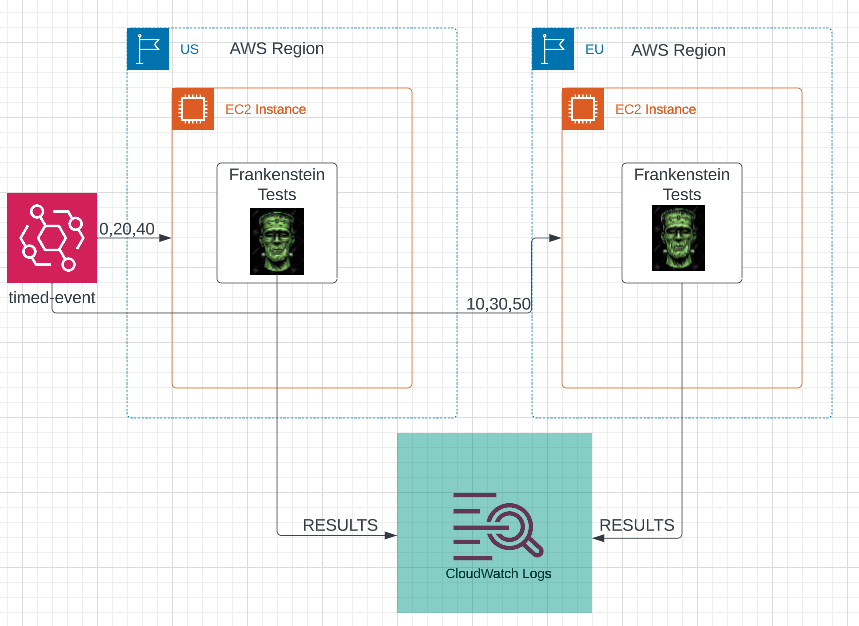
\includegraphics[width=\textwidth,height=\textheight,keepaspectratio]{./diagrams/frank_high_level.png}
  \caption{High level view of Frankenstein}
 \end{figure}
The components of a chatbot and each of its functions are created using microservice architecture. 
This is an architectural style that structures an application as a collection of services that are typically independently deployable and loosely coupled.
In essence its different parts can operate independently without being too dependent on each other.

\textit{The microservice architecture enables an organisation to deliver large, complex applications rapidly, frequently, reliably and sustainably - a necessity for competing and winning in today's world.}\autocite{Microservices}

Frankenstein runs tests against these micro services, testing the functions of the chatbot. They run several times an hour, every hour. 
\clearpage
\subsection{TestCafe}
The tests use a software package called Testcafe which is used for automated browser testing.  
By opening messenger in a browser in order to run the tests, it simulates what a user would do by interacting with a chatbot. 
If the chatbot reacts in the expected way the test passes, otherwise the issue is investigated and resolved.
\subsection{EC2}
The Frankenstein test suite is run on two \ac{EC2} instances, in two different \ac{AWS} regions, the US and the EU. 
EC2 instances are virtual machines where developers can define the resources they need to run their programs. For example, what regions they are to be run in and how much memory they need. 
\section{The Issue}
Running the tests causes a lot of contention for \ac{CPU} and memory. 
When a test run is instigated, all tests are competing for CPU usage because each EC2 instance is running thirty plus tests on one server which has limited memory.

Also there are numerous problems with Testcafe. 
\begin{itemize}
 \item ServisBOT finds Testcafe resource heavy, expensive and inefficient, causing slow CPU performance. 
 \item Because of competing resources some tests affect the performance of others. 
 \item Debugging and monitoring of Testcafe tests is complex, it uses a different syntax and approach to testing compared to other testing frameworks.
\end{itemize}

\section{Requirements for Bosco}

The main requirements for Bosco are listed as follows:
\begin{itemize}
  \item Create a new test runner that is more optimised, scalable, and cost-efficient than Frankenstein. 
  \item In particular, Bosco will focus on an automation tool called Puppeteer which has been proven by ServisBOT to be more performant than Testcafe. The Puppeteer package includes its own browser, Chromium, whereas Testcafe launches an external browser which is slow and cumbersome. With Puppeteer there is more control over what the developer can test, it is more efficient, easier to debug and has a lot more functionality. It is widely chosen by developers now. (4.6 million weekly downloads, 2023-03-02) \cite{Puppeteer}
  \item Implement an AWS Lambda, Step Function, State Machine which will run each test independently and can be scaled infinitely.
  \item Scheduled timed events will instigate test runs.
  \item The environment variables that Bosco will use will be retrieved from \ac{SSM} parameter store. 
  \item Bosco will have test profiles which can determine which tests are run in which regions and on which adapters. 
  \item Bosco will report the latest results of the test runs to Cloudwatch and store them in a DynamoDB table.
  \item Screenshots of failed test runs will be stored. 
\end{itemize}

\begin{figure}[ht]
 \centering
 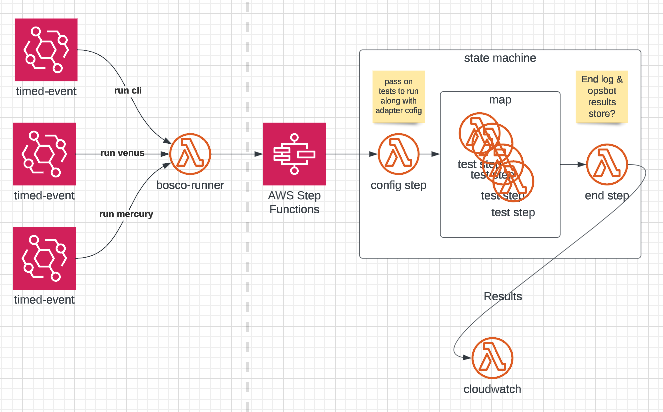
\includegraphics[width=\textwidth,height=\textheight,keepaspectratio]{./diagrams/bosco_high_level.png}
 \caption{High level view of Bosco}
\end{figure}

\chapter{Research and Development}

In order to determine the best approach, technologies and methodology for Bosco, the following research was carried out for the implementation of this project.

\begin{itemize}
 \item Cost analysis of Frankenstein
 \item Research into possible testing frameworks for Bosco
 \item Puppeteer comparison to Testcafe
 \item Lambda vs EC2 comparison
\end{itemize}

\section{Cost Analysis of Frankenstein Tests}

Cost analysis was carried out on Frankenstein which is evident in Figure \ref{frank:cost}. There are two EC2 instances running the tests in the EU and the US with two ServisBOT regions eu-private-1 and eu-1 in the EU and us-1 and usscif-1 in the US. 
All regions are in production except for eu-private-1 which is the testing region where most of the tests are run against before they are released to production. 
In summary a Frankenstein test run takes an average of six minutes \ref{tab:frank} which is costing ServisBOT on average \$20 per day for each region. 
This costs the company almost \$15,000 a year to run tests.

\begin{figure}[H]
 \centering
 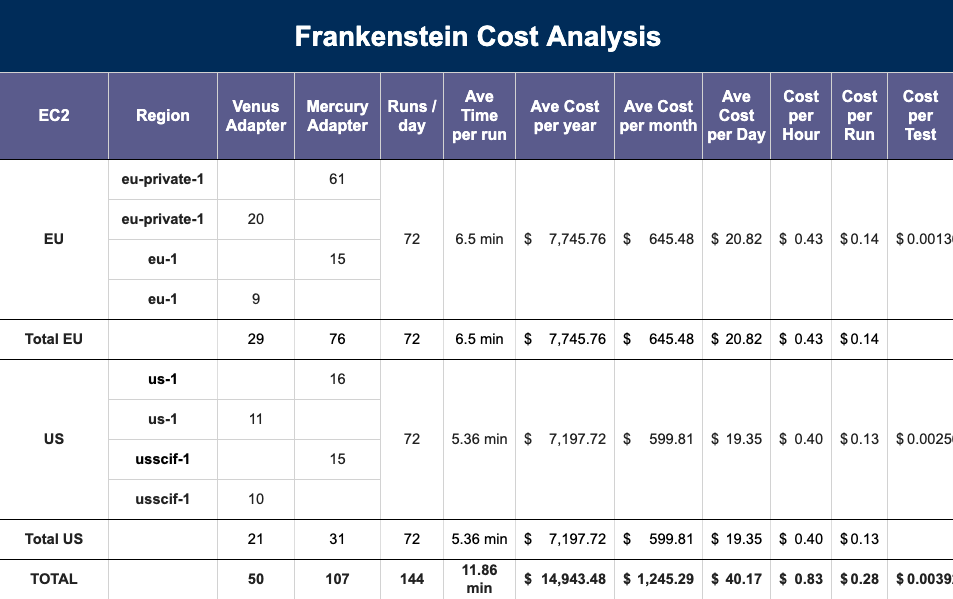
\includegraphics[width=\textwidth,height=\textheight,keepaspectratio]{./diagrams/frank_cost_analysis.png}
 \caption{Frankenstein Cost Analysis}
 \label{frank:cost}
\end{figure}

\section{Research into Possible Testing Frameworks for Bosco}

Frankenstein uses Mocha as its testing framework but there are multiple frameworks that ServisBOT could choose from. 
The following is an investigation into what else is available as well as a review of the current framework, Mocha.
\subsection{Mocha}

According to Mocha documentation, \textit{Mocha is a feature-rich JavaScript test framework running on Node.js and in the browser, simplifying asynchronous
testing. Mocha tests run serially, allowing for flexible and accurate reporting, while mapping uncaught
exceptions to the correct test cases.}\autocite{Mocha}

Asynchronous testing is used to verify code behaviour in software that relies on asynchronous programming. This programming allows tasks to be performed concurrently instead of waiting for each task to complete before moving on to the next one. 

Mocha, a testing framework, provides functions that execute in a specific order and logs results in the terminal. 
Mocha also cleans the software state to ensure that test cases run independently.

\begin{figure}[ht]
 \centering
 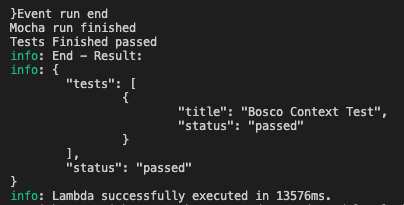
\includegraphics[width=0.75\textwidth,height=0.75\textwidth,keepaspectratio]{./diagrams/mocha_test_result.png}
 \caption{Mocha Test Result Output}
\end{figure}

\subsection{Jest}

Jest is a JavaScript testing framework created by Facebook. It is open source, well-documented and popular due to its
high speed of test execution. It comes with a test runner, but also with its own assertion and mocking library unlike Mocha where you need to install an assertion
library, there is no need to install and integrate additional libraries to be able to mock, spy or make assertions.

\subsection{Mocha vs Jest}

\begin{table}[ht]
 \centering
 \small
 \setlength\tabcolsep{6pt}
 \begin{tabular}{|c|c|c}
  \hline \textbf
  {Mocha}       & \textbf {Jest}\\
  \hline\hline
  Flexible configuration options & High Speed of Test Execution\\
  \hline
  Good Documentation       & Good Documentation\\
  \hline
  Ideal for back-end projects  & Test Runner included\\
  \hline
  Ad-hoc library choice     & Built in assertion and mocking library\\
  \hline
 \end{tabular}
 \caption{Mocha Vs Jest}
\label{table:mocha:jest}
\end{table}

\section{Puppeteer and Testcafe Comparison}

Puppeteer is a widely used test automation tool maintained by Google. Although it is not a dedicated test tool, it is popular for automating tasks such as web scraping and generating PDFs. 
In testing user flows within web applications, headful or headless browsers are used. A headless browser is a browser that is working in the background without a user interface and a heaful browser will automate the actions while displaying the browser. 
Headful browsers like Firefox with Selenium are slower but more reliable, while headless browsers like Testcafe sacrifice some reliability for speed.

Puppeteer aims to eliminate the need for developers to choose between speed and reliability when testing web applications. 
It does this by providing access to the Chromium browser environment, allowing developers to use either headless or headful browsers that run on the same platform as their users.
\subsection{Pros of using Puppeteer}

\begin{itemize}
 \item Simple to set up.
 \item Good documentation with lots of tutorials.
 \item Promise-based which is a software technique that is designed to manage tasks that do not occur in a specific order. It allows these tasks to happen simultaneously without any issues.
 \item Programmable web browser.
 \item Installs Chrome in a working version automatically.
 \item Puppeteer has a thin wrapper which provides a simpler interface for an underlying complex system.
 \item Bi-Directional (events) \- automating console logs is easy.
 \item It uses JavaScript first, which is one of the most popular programming languages.
 \item Puppeteer also gives you direct access to the Chrome DevTools Protocol which allows for developers to feel like there are fewer moving parts.
 \item Works with multiple tabs and frames. 
 \item It has an intuitive API.
 \item Trusted actions which are events by a user, like hovers.
 \item End to end tests are very fast.
 \item Pro and Con: Stability, which means how often tests fail after being authored other than when detecting a real application bug. Puppeteer waits for certain things but has to wait manually for others. 
 \item Debugging: Can write and debug Javascript from an IDE\@.
\end{itemize}

\subsection{Cons of using Puppeteer}
\begin{itemize}
 \item Limited cross-browser support, it only supports Chrome and Firefox.
 \item Feels like an automation tool and not a test framework. Often developers have to re-implement testing-related tools.
 \item Grids (running concurrently) in production are often a challenge.
 \item The automatic browser set-up downloads Chromium and not Chrome and there are subtle differences between the two.
 \item Smarter locators: No support for selecting elements in multiple ways.
 \item The software lacks the ability to run tests simultaneously on multiple computers, which can cause inefficiencies when testing large applications.
 \item The software cannot improve or fix test issues automatically, requiring manual intervention to correct problems.
 \item Does not support Autonomous testing which is testing without code or user intervention.
\end{itemize}

\subsection{Testcafe}

TestCafe is a Node.js tool to automate end-to-end web testing. It runs on Windows, MacOs, and Linux and
supports mobile, remote and cloud browsers (UI or headless). It is also free and open source.

\begin{table}[ht]
  \centering
  \small
  \setlength\tabcolsep{6pt}
  \begin{tabular}{|c|c|}
   \hline \textbf
   {Pros} & \textbf {Cons}\\
   \hline\hline
   Cross Browser Testing&Expensive\\
   \hline
   Open Source& Slow\\
   \hline
   Easy Setup \& Installation& Difficult to debug\\
   \hline
   Built-In Waits& No browser control\\
   \hline
   Supports devices without extra software package & Simulated events leads to false positives\\
   \hline
   UI End to End Testing\\
   \hline
   Both client and server side debug \\
   \hline
  \end{tabular}
  \caption{Pros and Cons of Tesfuncitontcafe}
 \end{table}

\begin{figure}{h}
 \centering
 \subfloat[\centering Npm Downloads]{{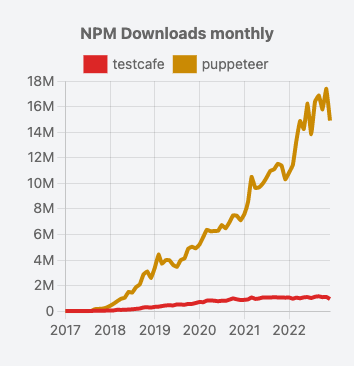
\includegraphics[width=5cm]{./diagrams/npm_pupp_tc}}}
 \qquad
 \subfloat[\centering GitHub stars]{{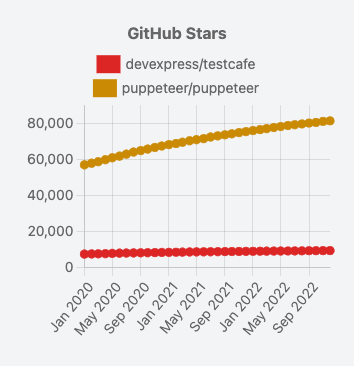
\includegraphics[width=5cm]{./diagrams/github_stars}}}
 \caption{Puppeteer vs Testcafe NPM statistics}
\end{figure}

\section{Lambda and EC2 Comparison}

AWS Elastic Compute Cloud \ac{EC2} is basically a virtual machine called an instance. Users can create an instance and define
the resources necessary for the task at hand. For example the type and number of CPU, memory, local storage and scalability. EC2 instances
are intended for consistent, static operations and users pay a recurring monthly charge based on the size of the instance, the operating
system and the region. The instances run until they are deliberately stopped.

Lambda on the other hand is billed per execution and per millisecond in use with the amount of memory the user allocates to the function.
When a lambda function is invoked, the code is run without the need to deploy or manage a \ac{VM}. It is an event based service that is
designed to deliver extremely short-term compute capability. AWS handles the back-end provisioning, loading, execution, scaling and unloading of the user's code.
Lambdas only run when executed yet are always available. They scale dynamically in response to traffic.

\begin{table}[ht]
  \centering
  \small
  \setlength\tabcolsep{6pt}
  \begin{tabular}{|c|c|c|}
   \hline
   \textbf{Feature} & \textbf{Lambda} & \textbf{EC2}\\
   \hline\hline
   Time to execute&milliseconds&seconds to minutes\\
   \hline
   Billing increments& 100 milliseconds&1 second\\
   \hline
   Configuration&Function& Operating System\\
   \hline
   Scaling Unit&Parallel function executions&Instances\\
   \hline
   Maintenance& AWS&AWS and User\\
   \hline
  \end{tabular}
  \caption{Comparison of AWS Lambda and EC2 \autocite{inbook}}
 \end{table}

\section{Conclusion}
After conducting research and analysis, it was affirmed that ServisBOT's decision to use Puppeteer in conjunction 
with Mocha, will provide greater control, reliability, and ease of use for developers. Mocha is more suitable for backend development and large projects than Jest. 
It allows the team to choose their own assertion library and is a more flexible and customisable framework.
Puppeteer is the chosen automation tool by developers now, mainly for its performance, reliability and ease of use.

Together with migrating the test runner from EC2 to Lambda, the test suite will become infinitely scalable and 
more cost efficient. Replacing Frankenstein with Bosco will mean that issues encountered by Frankenstein can be resolved and unnecessary costs (for 
example running too many tests) can be eliminated.

\chapter{Design \& Analysis}

\section{Proof of Concept - Running Puppeteer on a Lambda}

In order to prove it was possible to run Puppeteer tests on AWS Lambda, a basic end to end test was designed
to run with Puppeteer. This automated a scenario whereby a browser was launched with the URL of the
messenger page. After the page loaded, the messenger button was toggled and the chatbot displayed. The test
passed if the response from the messenger returned the expected output text.

\subsection{Mocha}

Mocha was incorporated as the testing framework. Assertions are made using the Assert library package and logged to the console but it is not in essence a testing tool.
Once mocha was configured and run without errors the next step was to run the script in a lambda.

\begin{figure}[H]
 \begin{tcolorbox}
  \begin{minted}[breaklines]{javascript}
  // basic-puppeteer.js
  const puppeteer = require('puppeteer');
  const URL = 'https://www.google.com';
  async run () => {
   const browser = await puppeteer.launch();
   const page = await browser.newPage();
   await page.goto(url);
   await page.screenshot({path: "screenshot.png"});
   browser.close();
  }
  run();
\end{minted}
\end{tcolorbox}
\captionof{figure}{Example of a function written with Puppeteer which takes a screenshot of the Google homepage and stores it locally}
\end{figure}
However, there are problems running Puppeteer in a lambda. Lambda has a 50 MB limit on the zip file you can upload. 
Due to the fact that it installs Chromium, the Puppeteer package is significantly larger than 50 {MB}. This 
limit does not apply when uploaded from an \ac{S3} bucket but there are other issues. 
The default setup of some Linux distributions, including the ones used by AWS Lambda do not include the necessary libraries required to allow Puppeteer to function.

\subsection{Node Modules}

A developer named Hansen\autocite{Hansen}, developed a work-around for this in the form of the node modules, \textit{puppeteer-core} and \textit{chrome-aws-lambda}.
Both these modules installed allow for a version of Chromium that is built to run for AWS Lambda. Incorporating
these ensured the tests ran successfully. Unfortunately these modules need to be in parallel with each other.

The \textit{aws-chrome-lambda} module has not been updated since June 2021 so its latest version is 10.1.0 whereas
\textit{puppeteer-core} has been updated regularly and at time of writing (26/03/23) is at version 19.8.0. When the version numbers are
synced the lambda function passes. Therefore using the latest version of both modules would mean they are incompatible with each other.

Regardless of the reason for these modules not being updated, relying on them is impractical and will eventually lead to the tests being broken.

\subsection{Docker}
 
A Docker container is a self-contained piece of software that packages up all the code and its dependencies needed to run an application. 
This ensures that the application runs reliably and consistently across different computing environments, even during different stages of development or on different computers with different settings. 
Using Docker containers instead of node modules can help to condense the code and simplify the application's setup.
\begin{figure}[H]
  \centering
  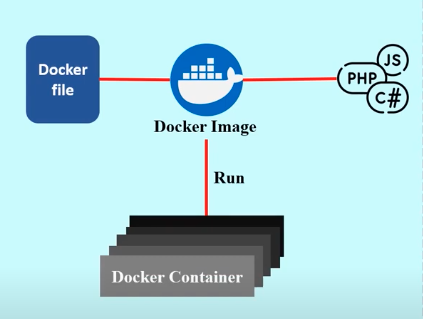
\includegraphics[width=10cm]{./diagrams/dockerexplained.png}
  \captionof{figure}{Illustration of Docker}
 \end{figure}

\subsection{Conclusion}
The puppeteer test was run locally in a Docker engine. When the test was functioning as expected the code was zipped up into docker image and got pushed to an AWS repository. 
The image was then deployed to the Bosco test-runner container where it was run and tested.
This significantly sped up the testing process, running a test in as little as six seconds.
This process provides more control over the testing environment and can target specific tests through the event handler input parameters.
The results validate the feasibility of running tests in a Lambda environment using Puppeteer.

\section{Stepfunction Design and Analysis}

The use of a Step Function in order to run the tests was considered by ServisBOT to be a viable option for Bosco. 
A step functions is a workflow that can be created through a sequence of lambda functions with each step being a state within
the workflow. It is based on a state machine and tasks, where a state machine is the workflow and a task is a
state in that workflow that another AWS service performs.

\begin{figure}[H]
 \centering
 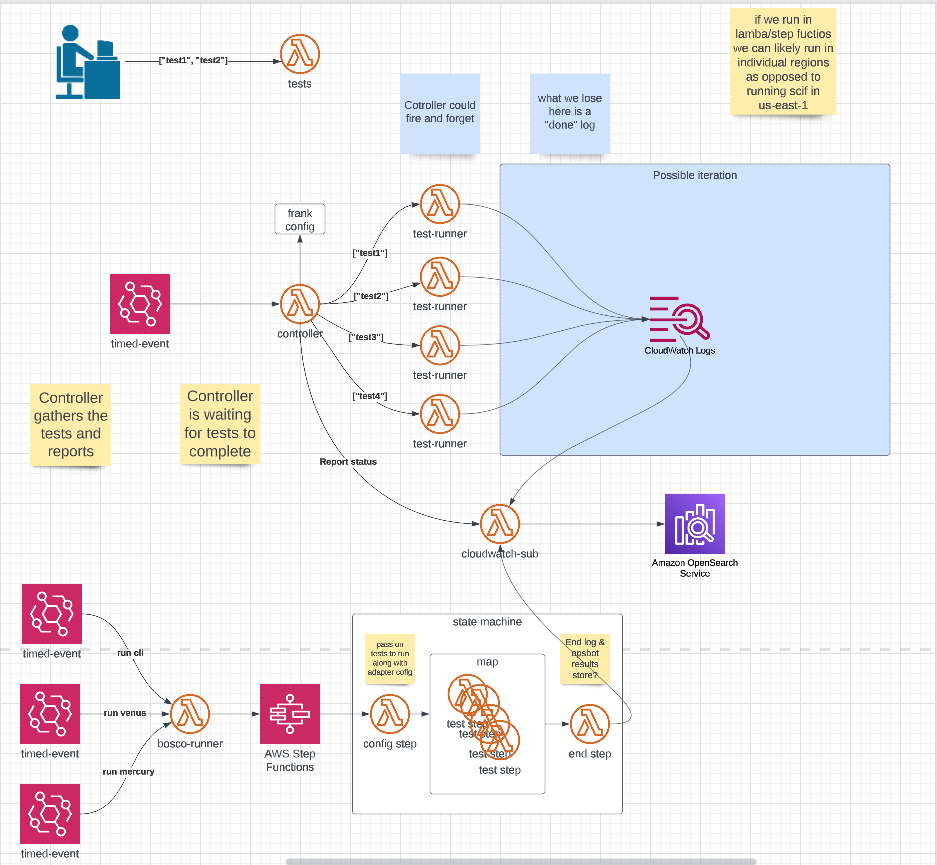
\includegraphics[width=15cm]{./diagrams/possible_implementation}
 \captionof{figure}{Bosco Initial Possible Implementations}
\end{figure}

\subsection{State Machine Transitions}

The Bosco test suite runs through five state transitions. 
\begin{enumerate}
  \item Start 
  \item StartState 
  \item Map 
  \item Done 
  \item End 
\end{enumerate}
In addition to these five transitions there is a transition per test that is run in the \textbf{Running} state. 
For example three tests, there are eight states as the \textbf{Running} state is executed three times. 

The first state is the \textbf{Start} state which initiates the run and then the \textbf{StartState} is invoked, creating an array of tests and passing the payload to the \textbf{Map} state.

Bosco uses an Inline Map state which is suitable for fewer than forty parallel iterations which is appropriate for Bosco at this time. 
The object structure passed to the \textbf{Running} lambda has been designed to enable the running of an array of tests or a single test, providing flexibility for the team to add tests as needed.

The lambdas run in parallel with each other with the results of the tests outputted to the \textbf{Done} lambda function which process the results. The \textbf{End} state completes the workflow.

\begin{figure}[H]
 \centering
 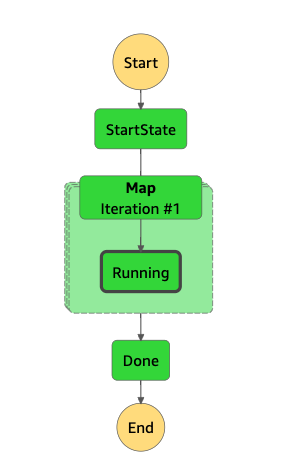
\includegraphics[width=5cm]{./diagrams/step_function}
 \caption{Bosco State Machine}
\end{figure}

\begin{figure}[H]
 \centering
 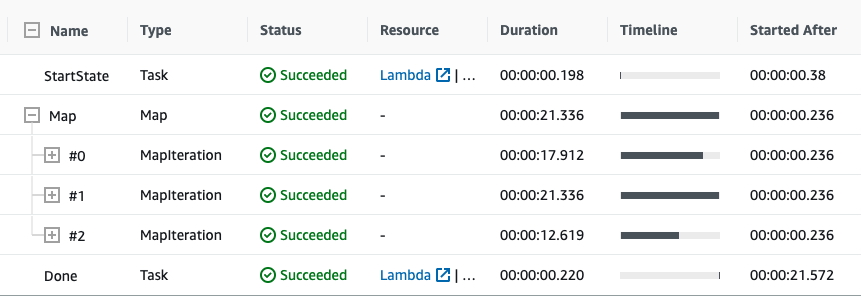
\includegraphics[width=15cm]{./diagrams/tablestepfx.png}
 \caption{Results of Execution of State Machine}
\end{figure}

\clearpage
\section{Cost Analysis of Bosco Step Function State Machine}

The cost of running the test suite in a state machine using AWS Step Functions was based on the number of state transitions.\autocite{Amazon} 
This cost analysis does not account for error handling, which may increase the cost due to retries. The cost per transition is \$0.000025 according to the AWS pricing calculator. 
The analysis was based on the current number of Frankenstein tests and the frequency they are run (three times an hour), which at the time of conducting the cost analysis may vary for Bosco tests.
This analysis is soley based on state machine transitions and does not account for other costs that Bosco may incur.

\begin{figure}[H]
 \centering
 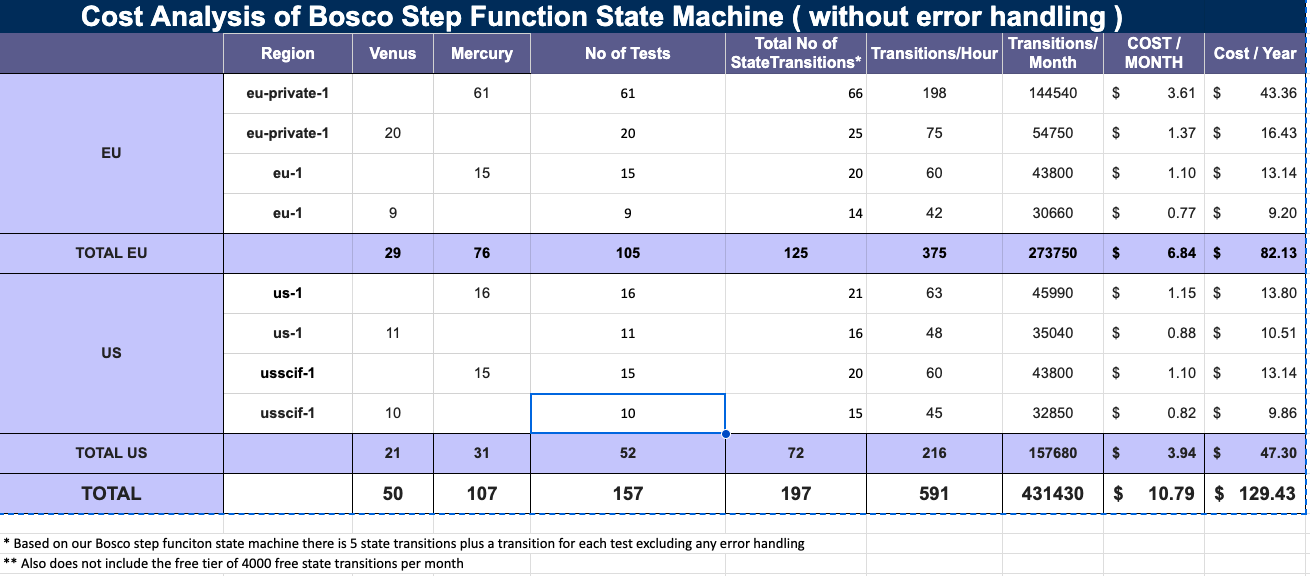
\includegraphics[width=15cm]{./diagrams/sfcost}
 \caption{Bosco Step Function Cost Analysis}
\end{figure}

\chapter{Bosco Implementation}
\section{Lightning Page}
The implementation of Bosco began after finalising the proof of concept. 
The first step involved creating a LightningPage class which is a utility class for testing the web page with the chatbot or messenger widget. 
It is the page the Bosco tests are running against and contains various functions that interact with the page's messenger widget. 
The class serves as the source for accessing the selectors and functions that have been added specifically for the Lightning page. 
Confining this functionality to a class reduces boilerplate code, a term for repetitive code. 
The tests were subsequently refactored to call the functions in the Lightning Page.

\begin{figure}[H]
 \begin{tcolorbox}
  \begin{minted}{js}
  async getMessage(index) {
    const allMessages = await this.getAllMessages();
    return allMessages[index];
  }
  \end{minted}
 \end{tcolorbox}
 \caption{Example of getMessage Lightning Page function}
\end{figure}

\section{Tests}
Five tests were written during the design and implementation stage of Bosco. 
\subsection{Context Test}
The initial Frankenstein test that was migrated to Bosco was the Context test. 
This test establishes the context from the URL and verifies whether it is displayed along with the rest of the context in the messenger. 
It was a relatively simple test to tackle at the early stages of Bosco.

\subsection{Conversation Engaged Test}
The next test was the Conversation Engaged test. Whenever a user interacts with a bot, a goal is generated, which is a default or custom event that's tracked to measure the success of the bot's interactions.
At first, it was believed that this test would be simple, but changes were requested after a pull request was submitted for review, including removing nested if statements and improving the code's formatting.

This created a need to parse the exported goal \ac{JSON} result. However, an error was encountered in the Servisbot \ac{CLI} proxy, where the outputted JSON was not formatted correctly and could not be parsed. 
To work around this, the \ac{CSV} output option was used instead of JSON and the \textit{csv-parse} node module was imported.

\subsection{Interaction Test}
This is a test designed to check the functionality of a multi-select list node in a chatbot.

\subsection{NLP Worker Lex V2 Intent Publish Test}
The \ac{NLP} Worker Lex V2 test uses a secret. Secrets can be defined as secure documents containing access keys, api keys, api secrets or IDs to external systems. 
They can be created and stored in the ServisBOT system and then referenced by bots securely. 
This is how ServisBOT manage \ac{API} keys for AWS\@.

A \textbf{Lex} worker is a remotely managed NLP worker which takes input and sends it to a Lex bot for Natural Language Processing. 
A Lex bot is an Amazon bot, users use ServisBOT to access, manage and run their Lexbots. 
\ac{NLP} is a form of \ac{AI} that transforms text that a user submits into language that the computer programme can understand. 
In order for ServisBOT to classify utterances using a remotely managed NLP, the correct API keys, access tokens or cross account roles need to be configured in the ServisBOT Secrets Vault.

An AWS cross account role is required in order to access Lex. An environment variable was created that the test could access called LEX\_V2\_CROSS\_ACCOUNT\_ROLE\_SECRET and to this was assigned the secret definition in JSON format. 

This test creates a long-living bot which is a bot that is created the first time the test is run and then reused for every test. 
The bot has a variable intent which is updated with a timestamp every time to ensure the bot is publishing successfully. 
When the bot is publishing its status is polled every 5 seconds until it succeeds and then the test starts.

\begin{figure}[H]
 \centering
 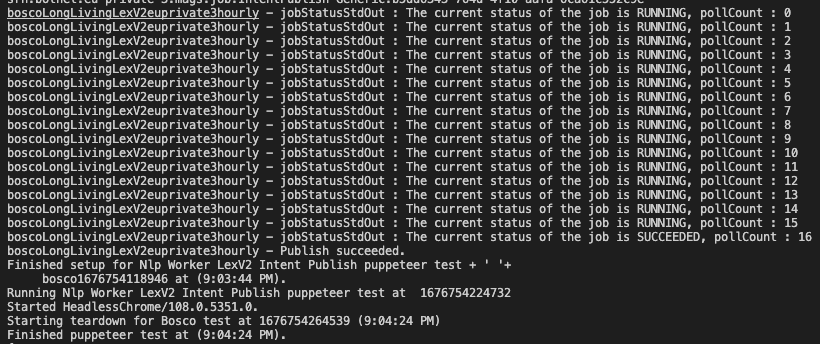
\includegraphics[width=15cm]{./diagrams/nlp_worker_poll.png}
 \caption{NLP worker test with polling}
\end{figure}

\subsection{CLI Test: Content}
Frankenstein also has a number of tests that test the functionality of the ServisBOT \ac{CLI}. The CLI has most of the functionality if not more of the ServisBOT UI. 
The tests do not use a web scraper like Testcafe as it is not needed. 
Instead the tests just run the cli commands and use an assertion to ensure they were carried out successfully. 

The CLI test chosen was the Content, create-describe-update-delete-list test. It was a basic test that tests a Content node by creating a content node object and then performing an update, describe and delete on it.

When the question of whether to incorporate CLI tests into Bosco was posed to the team, it was agreed that it was unnecessary to include the CLI tests. Bosco was to test Portal, specifically the \ac{UI} that the users would 
be using first hand. CLI tests are basically only for developers and there is less of a need to test them. The goal is to have full Frankenstein coverage with Bosco and testing the ServisBOT CLI proxy has 95\% coverage. 
The CLI test was removed from Bosco.

\section{CloudFormation}
When deploying Bosco, a  CloudFormation template in the form of YAML which is a human readable data language is run.  CloudFormation is an AWS service that allows developers to define and deploy infrastructure as code.
The Cloudformation template, which can be in either YAML or JSON format, is used to define and provision the AWS resources. When the CloudFormation template is uploaded to AWS it 
creates a CloudFormation stack which is a collection of AWS resources that can be managed as one unit. 
The template specifies the necessary environment variables, parameters, conditionals and other resources such as \ac{IAM} roles and policies. 

CloudFormation saves time and reduces errors as the same resources can be created multiple times once the template is defined.
A YAML formatting extension from Redhat to format the YAML file was used for Bosco as it is not possible to deploy the YAML unless the formatting is accurate.

Bosco's CloudFormation Template consists of the following resources:

\begin{description}
  \item [LambdaRole]: IAM (Identity and Access Management) role in AWS that is used to grant permissions to AWS Lambda functions.
  \item [ScheduledEventIAMRole]: IAM role used to grant permissions to the cron in Cloudwatch Events that will run the state machine.
  \item [BoscoIAMManagedPolicy]: AWS managed policy that defines the permissions for the roles and users attached to the IAM role.
  \item [ApiLambda]: The Lambda function that serves as an API endpoint for retrieving test run results from DynmaoDB.
  \item [TestOrchestrationLambda]: The Lambda function that configures the input to the state machine based on the profile provided in the event.
  \item [TestRunnerLambda]: The Lambda function that runs the suite of tests and returns the results.
  \item [TestResultsLambda]: The Lambda function that processes, stores and logs the test results.
  \item [StateMachine]: The AWS Step Function State Machine that is used to manage the orchestrator, runner and results Lambdas in a workflow based on a map inline state. 
  \item [ApiGateway]: The API Gateway created to access the DynamoDB results table.
  \item [ResultsDynamoTable]: The DynamoDB table that the results are written to.
  \item [S3BucketScreenshots]: The S3 bucket that screenshots of failed tests are stored in.
\end{description}

\section{Test Profiles}
One significant way in which Bosco differs to Frankenstein is in its capacity to define test profiles. 
Frankenstein is built to run all the tests, all the time. By creating a test profile it is possible to specify which 
environment, region and frequency of the tests which Frankenstein does not have the ability to do. 

A profiles folder was created which stores all the profiles defined by the ServisBOT region and the adapters Venus and Mercury in the Dev environment. 

\begin{figure}[H]
  \begin{tcolorbox}
   \begin{minted}{json}
    {
      "profile": "eu-private-3-venus",
      "organization": "bosco",
      "sbRegion": "eu-private-3",
      "awsRegion": "eu-west-1",
      "messengerUrl": "some-url",
      "testConfig": {
        "..."
      },
      "testSuite": [
        "..."
      ]
    }
   \end{minted}
  \end{tcolorbox}
  \caption{Sample Profile: eu-private-3-venus}
 \end{figure}

Each profile contains the testSuite so the orchestrator needed to be updated in order to read the file paths from the JSON provided in the 
event profile. The node module \textbf{file system(fs)} was used to read the contents of the profile. This was parsed to 
a javascript object and a spreader operator was used to combine the contents of the profile and the contents of 
the event inputted to the orchestrator and output these to the handler.

\begin{figure}[H]
 \begin{tcolorbox}
  \begin{minted}[breaklines]{javascript}
  const readProfile = fs.readFileSync(testProfile, (err, data) => {
  if (err) throw err;
  });
  const profile = JSON.parse(readProfile);
  const output = { ...profile, ...event };
  \end{minted}
 \end{tcolorbox}
 \caption{Parsing a JSON string to a javascript object and use of the spreader (\dots) operator}
\end{figure}

\subsection{Singleton Class: TestRunnerConfig}
It was a requirement for Bosco that the test configuration would be passed from the profile to the tests. 
There was quite a lot of code build needed for this as Mocha is limiting in that it doesn't 
allow the passing of parameters to the tests. 

A singleton class was created to overcome this. A singleton class is a class that can only have one instance of 
itself. It is used when there is going to be no change or update to the object for the duration it is used. 
This would be the case with our tests as we would just be using the configuration for accessing the Lightning page to run the tests.

Initially the TestRunnerConfig took in the runner event and created an instance of itself. 
It had getters to get different variables from the event which at the time were just the profile, testConfig, testSuite and environment. 
The tests ran but now the aim was to remove process.env to set the variables and use an Environment class that instead reads the environment variables from the TestRunnerConfig.

An Environment class was created using the environment from the event. This could now be accessed in the tests by calling the getters from the Environment object.
\begin{figure}[H]
 \begin{tcolorbox}
  \begin{minted}[breaklines]{javascript}
const testRunnerConfig = TestRunnerConfig.getInstance();
const environment = testRunnerConfig.getEnvironment();
const params = {
organization: environment.getOrganization(),
username: environment.getUsername(),
password: environment.getPassword(),
region: environment.getSBRegion()
};
\end{minted}
 \end{tcolorbox}
 \caption{Replacing proccess.env with getters to an Environment class invoked by a singleton class, TestRunnerConfig}
\end{figure}

\section{Environment Variables}
The environment variables are made up of the credentials needed to log into the ServisBOT CLI, the Log Level and the SSM parameters for the Lex V2 test which uses an external service.  
Storing the log level in the environment variables allows for consistency across the application, better security, easier debugging and flexibility. 
The log level can be changed without changing the code.

Initially, the environment variables were passed to the Orchestrator through the event. Once this was proven to work, the environment variables became part of the profile. However, a more 
secure option was necessary so they were subsequently removed from the profile and stored in \ac{SSM} Parameter Store, an AWS service for storage, configuration, secrets and data management. 
More information on SSM parameter store in Bosco is provided at a later stage in this report.

Two more classes were constructed in addition to the Environment class in order to resolve the environment variables. 
\begin{description}
  \item[EnvironmentResolver:]A class with three functions: resolveEnvironment; resolveEnvironmentVariable; retrieveSSMParam
  \item[resolveEnvironmentVariables:]A class which takes in the test profile and uses this to return an array of environment variables.
\end{description}

\begin{figure}[H]
  \begin{tcolorbox}
   \begin{minted}{json}
    "environment": [
      {
        "name": "SB_CLI_CREDENTIALS",
        "value": {
          "username": "some-username",
          "password": "some-password"
        }
      },
      {
        "name": "LEX_V2_CROSS_ACCOUNT_ROLE_SECRET",
        "value": {
          "externalId": "some-externalId",
          "crossAccountRole": "some-cross-account-role"
        }
      },
      {
        "name": "LOG_LEVEL",
        "value": "INFO"
      }
    ],
 \end{minted}
  \end{tcolorbox}
  \caption{Environment Variables Inputted to Handler}
 \end{figure}

The environment variables are provided to the handler at the same level as the \textit{testSuite} and the \textit{testProfileConfig}. 
By fetching and resolving the environment variables in the Orchestrator, this allows for a shared environment between the tests rather 
than providing the environment to each test which would be inefficient and resource heavy. Environments can grow and so this allows 
for flexibility in the development of Bosco.

It was essential to prove it was possible to flip between environments by either providing the environment to the
Orchestrator Lambda or by inputting it to the State machine as an event. 
This was important to prove because providing the state machine with the environment variables and testSuite configuration there is more control over the state
machine. What tests are run with what environment variables can be determined at any stage.

The state machine was then refactored to use a shared environment instead of
passing the environment variables in with each test object. In the state machine definition there is an option to
use an ItemSelector which allows the map to iterate over the ItemsPath but use the ItemSelector to add additional
parameters.

The updated definition of the state machine included the following extra parameters:

\begin{figure}[H]
 \begin{tcolorbox}
  \begin{minted}{json}
  {
    "ItemsPath":"$.testSuite",
    "ItemSelector": {
      "testSuite.$": "$$.Map.Item.Value",
      "environment.$": "$.environment",
      "testProfileConfig.$": "$.testProfileConfig",
      "executionId.$": "$$.Execution.Id"
    },
  }
\end{minted}
 \end{tcolorbox}
 \caption{State Machine Definition passing the environment to the Handler}
\end{figure}

The input to the Handler became the following:

\begin{figure}[ht]
 \begin{tcolorbox}
  \begin{minted}{json}
    {
      "testProfileConfig": {
        "..."
      },
      "executionId": "...",
      "environment": [
        "..."
      ],
      "testSuite": {
        "tests": [
          {
            "path": "goals/puppeteer-conversation-engaged.js"
          }
        ]
      }
    }
\end{minted}
 \end{tcolorbox}
 \caption{Input to one Iteration of Map State with just the Test Path}
\end{figure}

\section{Endpoint Proxy}

Bosco needed to support both Mercury and Venus engagement adapters similar to Frankenstein. This was achieved through the endpoints whereby 
each endpoint is suffixed by the test profile name. When the endpoint is created instead of creating it uniquely with the timestamp, middleware 
in the form of an endpoint proxy would instead suffix the endpoint with the profile and thereby point the tests to the URL 
containing the endpoint proxy. 

To prove the tests were making network calls to either Mercury or Venus, the tests were slowed down, run in headful mode and 
the network tab examined. When the browser was talking to Venus there calls to \textbf{VendAnonConversation} and \textbf{ReadyForConversation} and when there were calls to Mercury, \textbf{graphql} calls were evident.

\begin{figure}[H]
 \centering
 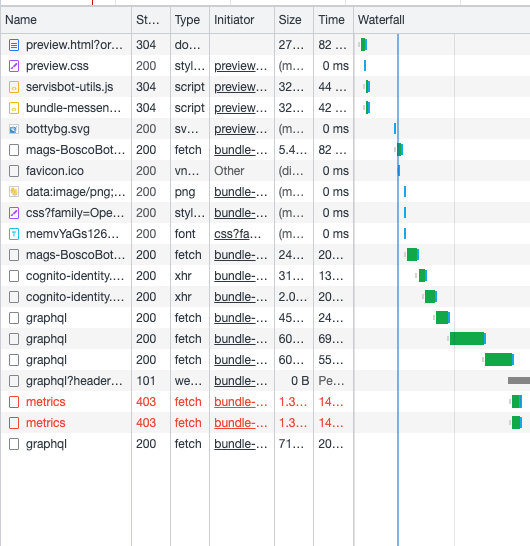
\includegraphics[width=15cm]{./diagrams/mercury_network_calls.png}
 \caption{Mercury Network Calls}
\end{figure}

\begin{figure}[H]
 \centering
 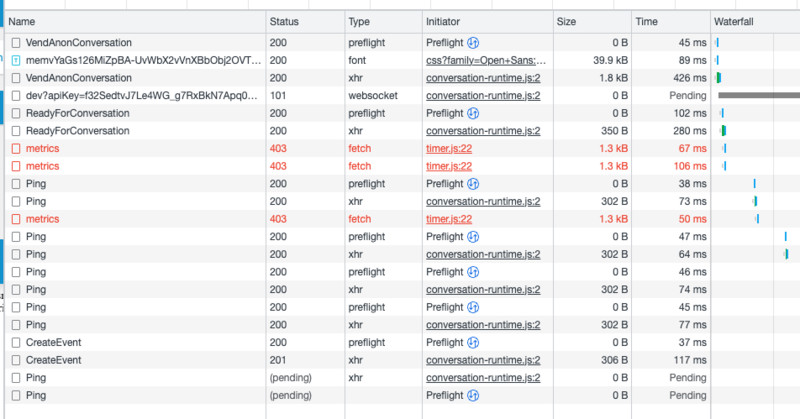
\includegraphics[width=15cm]{./diagrams/venus_network_calls.png}
 \caption{Venus Network Calls}
\end{figure}



\section{SSM Parameters}
In order for Bosco to build the environment in the orchestrator, SSM parameter store was utilised. 
\textit{SSM (Systems Manager) is a service provided by AWS that allows you to securely store and retrieve data for your application.}\autocite{Halley}.
They can be encrypted and the service is easy and free to use. 
A few lines of code can retrieve the parameters from the store. 

The steps to this task were as follows:
\begin{itemize}
\item The parameters were created in the SSM parameter store in the same format as the Frankenstein parameters.
\item Code was added to the orchestrator to read the SSM parameters using the \ac{aws-sdk}.
\item A new policy was added to the  CloudFormation template in order to give \ac{IAM} permissions to read from the parameter store
\item The environment was built in the orchestrator by retrieving the SSM parameters in the orchestrator, building the environment object and returning this in the output.
\item A Secrets was added in order to retrieve the SSM parameters from the parameter store to extract that work from the orchestrator. Later to be renamed EnvironmentResolver. 
\item The README was updated to reflect the changes for future development from the ServisBOT team.
\end{itemize}

\begin{figure}[H]
 \centering
 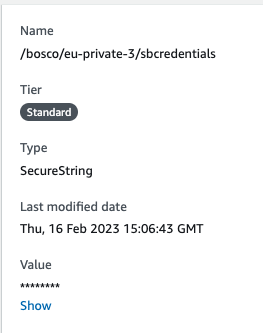
\includegraphics[width=8cm,height=8cm,keepaspectratio]{./diagrams/ssm_params.png}
 \caption{SSM Parameters created in AWS Systems Manager}
\end{figure}

\section{Eventbridge Rules (CRON) }

Like Frankenstein, Bosco needs to run on a scheduled event. AWS Eventbridge allows developers to trigger events on a CRON which is a command to an operating system or server for a job that is to be executed at a specified time. 
To trigger the state machine to run different profiles at different times, in different regions, the  CloudFormation file needed to be updated. 
\begin{itemize}
 \item Scheduled Rules were added as resources to the CloudFormation template.
 \begin{tcolorbox}
  \begin{minted}[fontsize=\footnotesize, breaklines]{yaml}
  MercuryProfileScheduledRule:
    Type: AWS::Events::Rule
    Properties:
      Name: !Sub "${CoreName}-Mercury-Profile"
      State: "ENABLED"
      ScheduleExpression: ScheduleVenusExpression
      Targets:
        - Arn: 
            Fn::ImportValue: 
              Fn::Sub: "${Environment}-bosco-StateMachineArn-${AWS::Region}"
          Id: !Sub "${CoreName}-Mercury"
          Input: !Sub '{"profile": "${ServisBotRegion}-mercury"}'
          RoleArn: 
            Fn::ImportValue:
              Fn::Sub: ${Environment}-bosco-ScheduledEventIAMRoleArn-${AWS::Region}
  \end{minted}
 \end{tcolorbox}
 \item The CRON rules were then added.
  \begin{tcolorbox}
   \begin{minted}[fontsize=\footnotesize, breaklines]{yaml}
   ScheduleMercuryExpression: { Type: String, Default: "cron(0,20,40 * * * ? *)" } # run at 0,20,40 past the hour
   ScheduleVenusExpression: { Type: String, Default: "cron(10,30,50 * * * ? *)" } # run at 10,30,50 past the hour
   ScheduleHourlyExpression: { Type: String, Default: "cron(0 * * * ? *)" } # run at 0 past the hour
   \end{minted}
  \end{tcolorbox}

 \item The triggers were added.
 \begin{tcolorbox}
  \begin{minted}[fontsize=\footnotesize, breaklines]{yaml}
   EuMercuryTriggerEnabled: !Equals [ !Ref MercuryEuRunnerEnabled, "true" ]
   EuVenusTriggerEnabled: !Equals [ !Ref VenusEuRunnerEnabled, "true" ]
   EuHourlyTriggerEnabled: !Equals [ !Ref HourlyEuRunnerEnabled, "true" ]
  \end{minted}
 \end{tcolorbox}
 \item A new Scheduled Event IAM role to execute the state machine was added with a special policy that allows the execution of the state machine. 
 
 \begin{tcolorbox}
  \begin{minted}[fontsize=\footnotesize, breaklines]{yaml}
    ScheduledEventIAMRole:
        Policies:
          - PolicyName: StateMachineExecutionPolicy
            PolicyDocument:
              Version: "2012-10-17"
              Statement:
                - Effect: "Allow"
                  Action: "states:StartExecution"
                  Resource:
                    - !Ref ImportBoscoStateMachine
  \end{minted}
 \end{tcolorbox}
\end{itemize}

Once the  CloudFormation file was deployed successfully, it was possible to observe the timed events executing successfully. The following table displays  
each execution, which is  given a unique ID and runs at regular intervals past the hour. 

The working CRON instigated state machine was showcased to the team and they were 
queried on whether they would like the introduction of a profile that runs hourly as opposed to every twenty minutes. 
The team agreed that the tests were already running too frequently with excessive costs. Bosco will have more control over what tests are run, in what regions and how frequently through the test profiles, therefore giving ServisBOT 
much more control over their testing suite and providing flexibility and control that Frankenstein seriously lacks in.

\begin{figure}[ht]
  \centering
  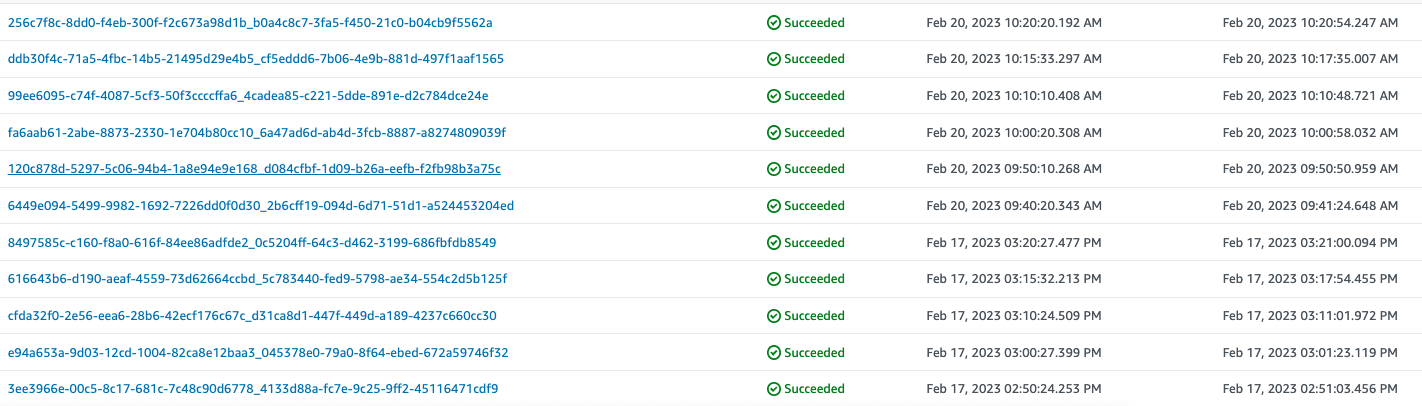
\includegraphics[width=15cm]{./diagrams/state_machine_cron_executions.png}
  \caption{State Machine Executions on a CRON }
 \end{figure}

\section{DynamoDB}
Bosco stores the latest test results of each profile in a global DynamoDB table. 
Each profile has a row in the table with details on the results of the latest test run. 
The attributes stored in the dynamo table are the duration, the end time and the status of the test run. 
When the Bosco state machine is run, the test results are stored in this table overwriting the previous test run as the team are only interested in the latest result.

\begin{figure}[ht]
  \centering
  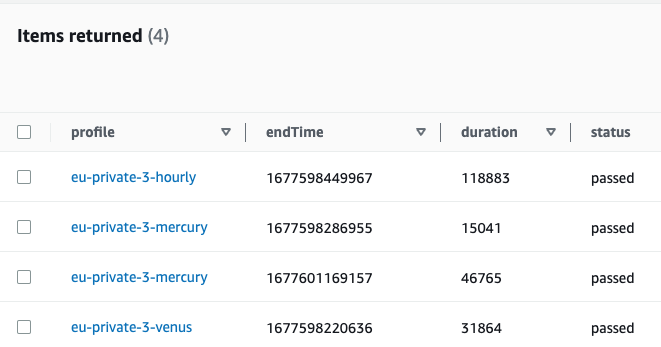
\includegraphics[width=15cm]{./diagrams/dynamodb.png}
  \caption{Dynamo DB Global Table Results}
 \end{figure}

The process to completing this task was the following:
\begin{itemize}
\item Manually creating a DynamoDB table in the development environment and deciding the attributes that would be written to it, namely \textbf{profile} would be the primary key and there would be no other key identifiers as it is only the latest result per profile Bosco will store.
\item The handler was then refactored in order to pass the profile, the endTime and the duration, along with the status to the results lambda. 
\item The results lambda then used the aws-sdk to write to the Dynamo DB. It filtered through the status of all the tests and if there was a failed test then the overall test run was marked as a fail.
\item Once the step function was writing to the table which was created manually, a new resource, a Global Dynamo table was added to the  CloudFormation template.
\item A condition was added to the Dynamo table so that it is possible to choose what profiles to deploy the table in.
\end{itemize}

\chapter{Deployment}
The deployment process was undertaken with help from the team as the initial plan needed to be altered. 
The CRON triggers which were initially in the CloudFormation template were removed and instead were put in a script specific to the AWS Region they would be deployed in which allowed for more control over what tests to run in what region. 

\section{\ac{CI/CD} Process}
\textit{CI/CD falls under DevOps (the joining of development and operations teams) and combines the practices of continuous integration and continuous delivery. CI/CD automates much or all of the manual human intervention traditionally needed to get new code from a commit into production, encompassing the build, test (including integration tests, unit tests, and regression tests), and deploy phases, as well as infrastructure provisioning. With a CI/CD pipeline, development teams can make changes to code that are then automatically tested and pushed out for delivery and deployment.}\autocite{CICD}

The steps to the CICD process for Bosco were as follows:

\begin{itemize}
  \item The developer puts in a \ac{PR} with the changes they made to the project code.
  \item A second developer reviews the code and when content with the changes, approves the merge.
  \item Developer merges the branch which initiates the CICD process. 
  \item Unit tests are run, artefacts are built and the project code is deployed in testing.
  \item If successful Slack will report on the Staging Releases channel, otherwise the error needs to be located and debugged. 
  \item The developer tests the code changes on testing.
  \item When the changes are verified, the developer tags a release through deploybot on Slack.
  \item This initiates the CICD process again which builds artefacts, runs unit tests, integration tests and deploys to the testing account again as a tagged release.
  \item The developer tests on testing again.
  \item Once verified, the developer requests a deploy to production from deploybot on Slack.
  \item Operations trigger the deployment, the CICD process is initiated once more with the project being deployed on production/upper.
  \item The developer tests the code on upper and verifies.
\end{itemize}

\section{Handling Multiple ServisBOT Regions}
It was required that Bosco would run multiple ServisBOT region test profiles per deploy. For example deploying an instance of 
Bosco in the AWS region, eu-west-1 should be capable of creating CRON schedules for ServisBOT regions, eu-1 and eu-private-1. 

\subsection{Triggers}
Triggers are what initiates the test runs. They can be defined for each region and each environment. The decision was taken 
to reduce the number of test runs that Frankenstein runs. Frankenstein runs 24/7 and this was deemed unnecessary. This will have a huge cost reduction 
effect on the company. The following times were decided on for the test runs.

\begin{table}[ht]
  \centering
  \small
  \setlength\tabcolsep{5pt}
  \begin{tabular}{|c|c|c|c|c|}
   \hline & \textbf{Staging/Lower}&\textbf{Prod/Upper}&\textbf{Prod/Upper}&\textbf{Prod/Upper}\\
   \hline\hline
   \textbf{ServisBOT Region}&\textbf{eu-private-1}&\textbf{eu-1}&\textbf{us1}&\textbf{usscif1}\\
   \hline
   \textbf{Timeframe}&Mon-Fri, 8am-5pm&24/7&24/7&24/7\\
   \hline
   \textbf{Mercury}&0,20,40&0,20,40&0,20,40&N/A\\
   \hline
   \textbf{Venus}&10,30,50&10,30,50&10,30,50&10,30,50\\
   \hline
   \textbf{Hourly}&hourly&hourly&hourly&hourly\\
   \hline
  \end{tabular}
  \caption{Scheduled Triggers (CRON)s for Running Bosco}
 \end{table}

A trigger was created in cloud formation for each AWS region and ServisBOT region pair.
For example:
\begin{itemize}
  \item src/triggers/eu-west-1/eu-1-triggers.yaml
  \item src/triggers/eu-west-1/eu-private-1-triggers.yaml
\end{itemize}
Within each of these template files is the infrastructure for the eu-1 CRON and eu-private-1 respectively.
A new lambda was created in Bosco which does the following:
\begin{itemize}
  \item When invoked, checks the AWS region the lambda is running in.
  \item Reads the src/triggers/<aws-region> folder, and uses the AWS SDK to deploy each of the templates found within this folder.
  \item The lambda function has the ability to poll to check for new or updated CloudFormation stacks.
  \item The lambda will fail if any of the stacks fail to create/update.
  \item post-build code build script invokes the lambda. This now only runs on deployment to an account (not the CICD account).
\end{itemize}

\section{Additional Features Post-Deployment}

\subsection{Logging Test Results}
A LogReporter class was added in order to report the test results to Cloudwatch. Each test reports on itself plus each test run will log a completion report. 
These reports can be viewed in Cloudwatch in the following format.

\begin{figure}[H]
  \begin{tcolorbox}
   \begin{minted}{json}
    {
      "SbRegion": "eu-private-3",
      "TestProfile": "eu-private-3-venus",
      "TestTitle": "Bosco Interaction Test",
      "DurationInMs": 42268,
      "Result": "passed",
      "Type": "test",
      "TestRunnerIdentifier": "1b3bc8b5-7db5-48ae-83a4-3ad40a6bfa92"
  }
 \end{minted}
 \end{tcolorbox}
 \captionof{figure}{Cloudwatch Log of Bosco Interacton Test}
 \end{figure}

 \begin{figure}[H]
  \begin{tcolorbox}
   \begin{minted}{json}
    {
      "SbRegion": "eu-private-3",
      "TestProfile": "eu-private-3-venus",
      "TotalDurationInMs": 120218,
      "Result": "passed",
      "Type": "completion",
      "TestRunnerIdentifier": "1b3bc8b5-7db5-48ae-83a4-3ad40a6bfa92"
  }
 \end{minted}
 \end{tcolorbox}
 \captionof{figure}{Cloudwatch Log of Complete Test Run}
 \end{figure}

 \subsection{Cloudwatch Insights}
 A query was constructed and added to the READMe to make it easier for developers to be able to view failed test results.
 The following figure is the result of the query. \ref{fig:insight}
 \begin{figure}[H]
  \centering
  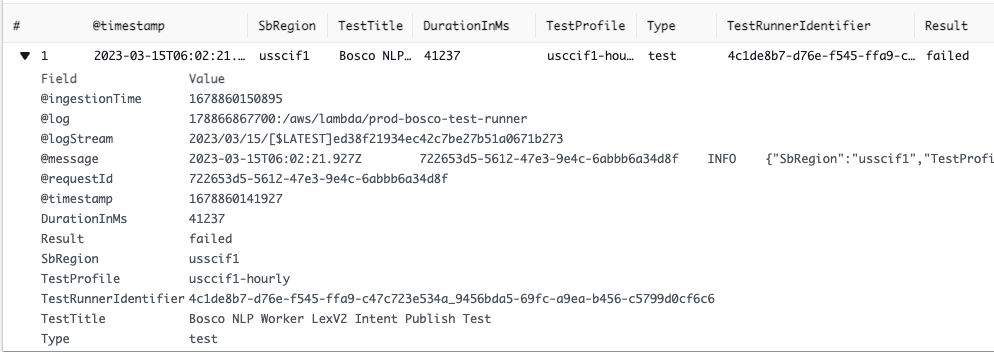
\includegraphics[width=\textwidth,height=\textheight,keepaspectratio]{./diagrams/insights.png}
  \caption{Cloudwatch Log Insight of Failed Tests for 1 week on Production}
  \label{fig:insight}
 \end{figure}

\subsection{Failed Test Screenshots stored in S3}
On failure of a test, a screenshot is taken using Puppeteer and stored locally in a /tmp/screenshots folder with the execution ID of the state 
machine run. On completion of the test run, the handler checks for the existence of a directory with the execution ID and if 
it exists then it uploads each screenshot in the directory to an S3 bucket. The /tmp directory is the only directory that lambda can access. 
Any attempts to read/write to other named directories will cause an error. 
Once the files have been uploaded the /tmp/screenshots directory is deleted.

The S3 bucket is only deployed in the testing environment but production and dev will all use this bucket. 
This is to save multiple buckets being deployed unnecessarily.

\begin{figure}[ht]
  \centering
  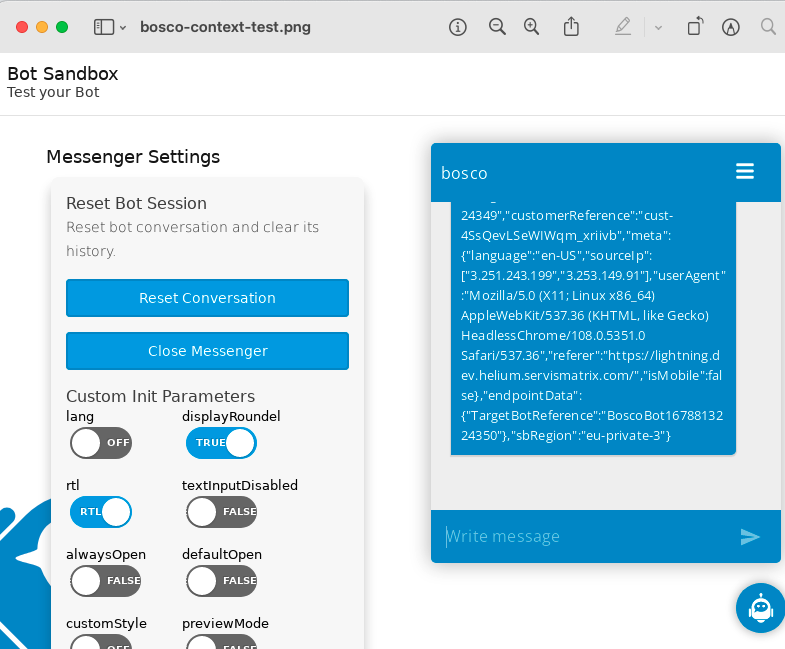
\includegraphics[width=\textwidth,height=\textheight,keepaspectratio]{./diagrams/screenshot.png}
  \caption{Screenshot of failed test}
 \end{figure}

\chapter{Conclusion}
\section{Reflection}
The ServisBOT testing process will significantly benefit from the addition of Bosco, as it will streamline and enhance the testing procedure, leading to quicker and more effective outcomes.
The project was developed to address limitations of the previous testing framework, Frankenstein which it has successfully achieved.
The use of Puppeteer in Bosco allows for more accurate and realistic testing of the ServisBOT Portal UI, while also improving the speed of the tests.

Running the tests on Lambda instead of EC2 provides several advantages for the Bosco project. 
\begin{itemize}
  \item One of the most significant improvements is the increased scalability and flexibility which will allow the team to add tests and run them in parallel with each other instead of the tests competing for resources. 
  \item Additionally, Lambda can be easily integrated with other AWS services, such as S3 and CloudWatch, which provides a more streamlined and automated testing process.
  \item While the exact reduced cost of running the tests at this time cannot be determined, there is strong indications that running tests on Lambda will be more cost-effective than using EC2 instances.
  \item One of the main reasons why running tests on Lambda was a vast improvement over EC2 was the faster and more reliable performance. Lambda functions can be invoked in milliseconds which allows for faster test execution and improved overall test cycle time. A test run can now be executed in under a minute compared to six minutes for Frankenstein. 
Theoretically, the Step Function will take as long as the longest Mocha test event whether that contains one test or a number of tests. 
\item Furthermore, Lambda provides high availability and fault tolerance, which means that tests are less likely to fail due to infrastructure issues or downtime.
\end{itemize}

In summary, the development of Bosco has been a demanding but rewarding experience that has provided valuable insights into AWS Lambda, CloudFormation, and related services. 
The seamless execution of tests on the Lambda function and the significant cost savings compared to EC2 were gratifying. 
Despite uncertainty regarding the actual cost, Lambda's cost-effectiveness is assured. 
The Bosco test runner has been seamlessly integrated into the development workflow and has demonstrated its efficacy in testing the ServisBOT Portal UI. 
Overall, contributing to ServisBOT's platform quality and reliability through Bosco has been a source of pride.
\section{Key skills}
\begin{itemize}
  \item Sprint planning. 
    \begin{itemize}
      \item Using Jira for creating sprints.
      \item Creating tickets/tasks for the project.
      \item Pointing the tickets. Estimating how long they will take based on their complexity.
      \item Keeping track of progress on each ticket and sprint.
    \end{itemize}
  \item Amazon Web services. In particular:
    \begin{itemize}
      \item Lambda 
      \item Step Functions 
      \item CloudFormation 
      \item S3 
      \item DynmaoDB 
      \item AWS regions 
      \item SSM Parameters
      \item IAM
      \item Codebuild
      \item Cloudwatch
    \end{itemize}
  \item Showcasing remotely the progress of the project to the team.
  \item Isolating code to test it. Providing the desired input and testing a small script until the desired output was achieved.
  \item Removing boilerplate code
  \item Eliminating nested loops
  \item Using Docker containers
  \item CICD process
  \item Git
  \item Javascript fundamentals
  \item Project design and infrastructure
  \item Puppeteer and Mocha
  \item Academic Writing
  \item Latex
\end{itemize}
\section{Challenges}
Fortunately the team at ServisBOT were very supportive and as a result, working on this project posed very few challenges. 
Most of the challenges that were faced were with regards to inexperience working on such a complex project and practical knowledge of software design.
The following list iterates some of the challenges that were encountered.
\begin{itemize}
  \item It became obvious early in the process that the fundamentals of Javascript and object oriented programming were still challenging and not fully comprehended. However, from being assigned new tasks every week, which explored 
  various components, AWS services, features and technologies, a steep learning curve was overcome and skills were achieved at a pace which inevitably sped up the process.
  \item As this was a work based project which was completed during an internship, the code had to be reviewed by a team member before being approved. If the team was under pressure this could take a few days which disrupted the workflow.
  \item The complexity of the project was incredibly challenging. Although given time to move at a pace that was reasonable, trying to understand all the different components of Bosco was often overwhelming.
  \item Mastering Puppeteer. Accessing the selectors on the Lightning page was tricky in comparison to Testcafe which uses a variety of methods to access the elements and is in reality more straightforwardward and easier to read.
  \item Passing data through the State Machine in the format required by ServisBOT. It was time consuming to test the state machine and tricky to figure out how to pass parameters. Despite extensive documentation, it was challenging to find resolutions specific to Bosco. 
  \item Learning how to use LateX for the project report initially was very confusing and stunted the process. It was not a requirement but a personal challenge that was undertaken. 
\end{itemize}
\section{Future Work}
\subsection{Migrating the Remainder of the Tests}
At the end of the project, Bosco is at a state where the rest of the team can now add the remainder of the tests. 
There are in total thirty Frankenstein Testcafe tests of which four are already transitioned to Bosco. Any team member once lightly versed in Puppeteer and Mocha can now transition easily. 
Bosco is running in production and testing the four tests that were written during this project. The tests in Frankenstein will be turned off one by one as 
they are migrated to Bosco. 

\subsection{API}
Currently an API for Bosco is being developed which will retrieve the latest test results for the DynamoDB table. 
Tests have been developed to health check the routes of this API. 

\subsection{Alert of Test Failures}
Alerts that are reported to the Slack channel are yet to be developed.

Bosco will continue to be a work in progress for the ServisBOT team. 
The tasks related to Bosco will be migrated to the Core team's planning board as the entire team will take over the development of Bosco. 

\appendix
\chapter{Methodology}
Jira was used to keep track the sprints on the Bosco project. Week long sprints were the chosen method for the implementation phase as this
was better suited to the type of project as the urgency to have it complete is high.

The projcet was broken into three Epics:

\begin{itemize}
  \item Bosco Research and Design
  \item Bosco Implementation
  \item Bosco Dissemination Phase
\end{itemize}
\section{Research and Design}
Research and Design was carried out over a number of weeks starting in December with the main focus on the following:
\begin{itemize}
\item Review Puppeteer
\item Review Lambda
\item Initial Step Function R\&D
\item Cost Analysis
\end{itemize}

\section{Implementation}
The implementation of Bosco was carried out in one week sprints as was required by the project supervisor in ServisBOT\@. 
\subsection*{Sprint 1}
\begin{itemize}
\item Add two Frankenstein tests to Bosco
\item Step Function Lambda code moved to Bosco
\end{itemize}

\subsection*{Sprint 2}
\begin{itemize}
\item Cloudformation
\end{itemize}

\subsection*{Sprint 3}
\begin{itemize}
\item Bosco environment variables for tests
\item Refactor state machine to use a shared environment
\end{itemize}

\subsection*{Sprint 4}
\begin{itemize}
\item Test profiles and overrides
\end{itemize}

\subsection*{Sprint 5}
\begin{itemize}
\item Create a test with a secret
\end{itemize}

\subsection*{Sprint 6}
\begin{itemize}
\item Lightning URL in tests needs to be config in test profiles
\end{itemize}

\subsection*{Sprint 7}
\begin{itemize}
\item READMe update for Developer Experience
\item Schedule different test profiles to run on a CRON
\item Orchestrator builds the Environment
\end{itemize}

\subsection*{Sprint 8}
\begin{itemize}
\item Create a CLI test in Bosco
\item Staging organization and SSM Parameters
\end{itemize}

\subsection*{Sprint 9}
\begin{itemize}
\item Deployment of Bosco
\item Storing Test Results in Dynamo DB
\item Logging Test Results and Completion
\item Bosco infrastructure to handle multiple ServisBOT regions with one deploy
\end{itemize}

\subsection*{Sprint 10}
\begin{itemize}
\item Screenshots of failed tests upload to S3
\item Api to serve latest test results \textit{(In Review)}
\item Alert of test failures and failed test runs \textit{(Not Complete)}
\end{itemize}

\begin{figure}[ht]
 \centering
 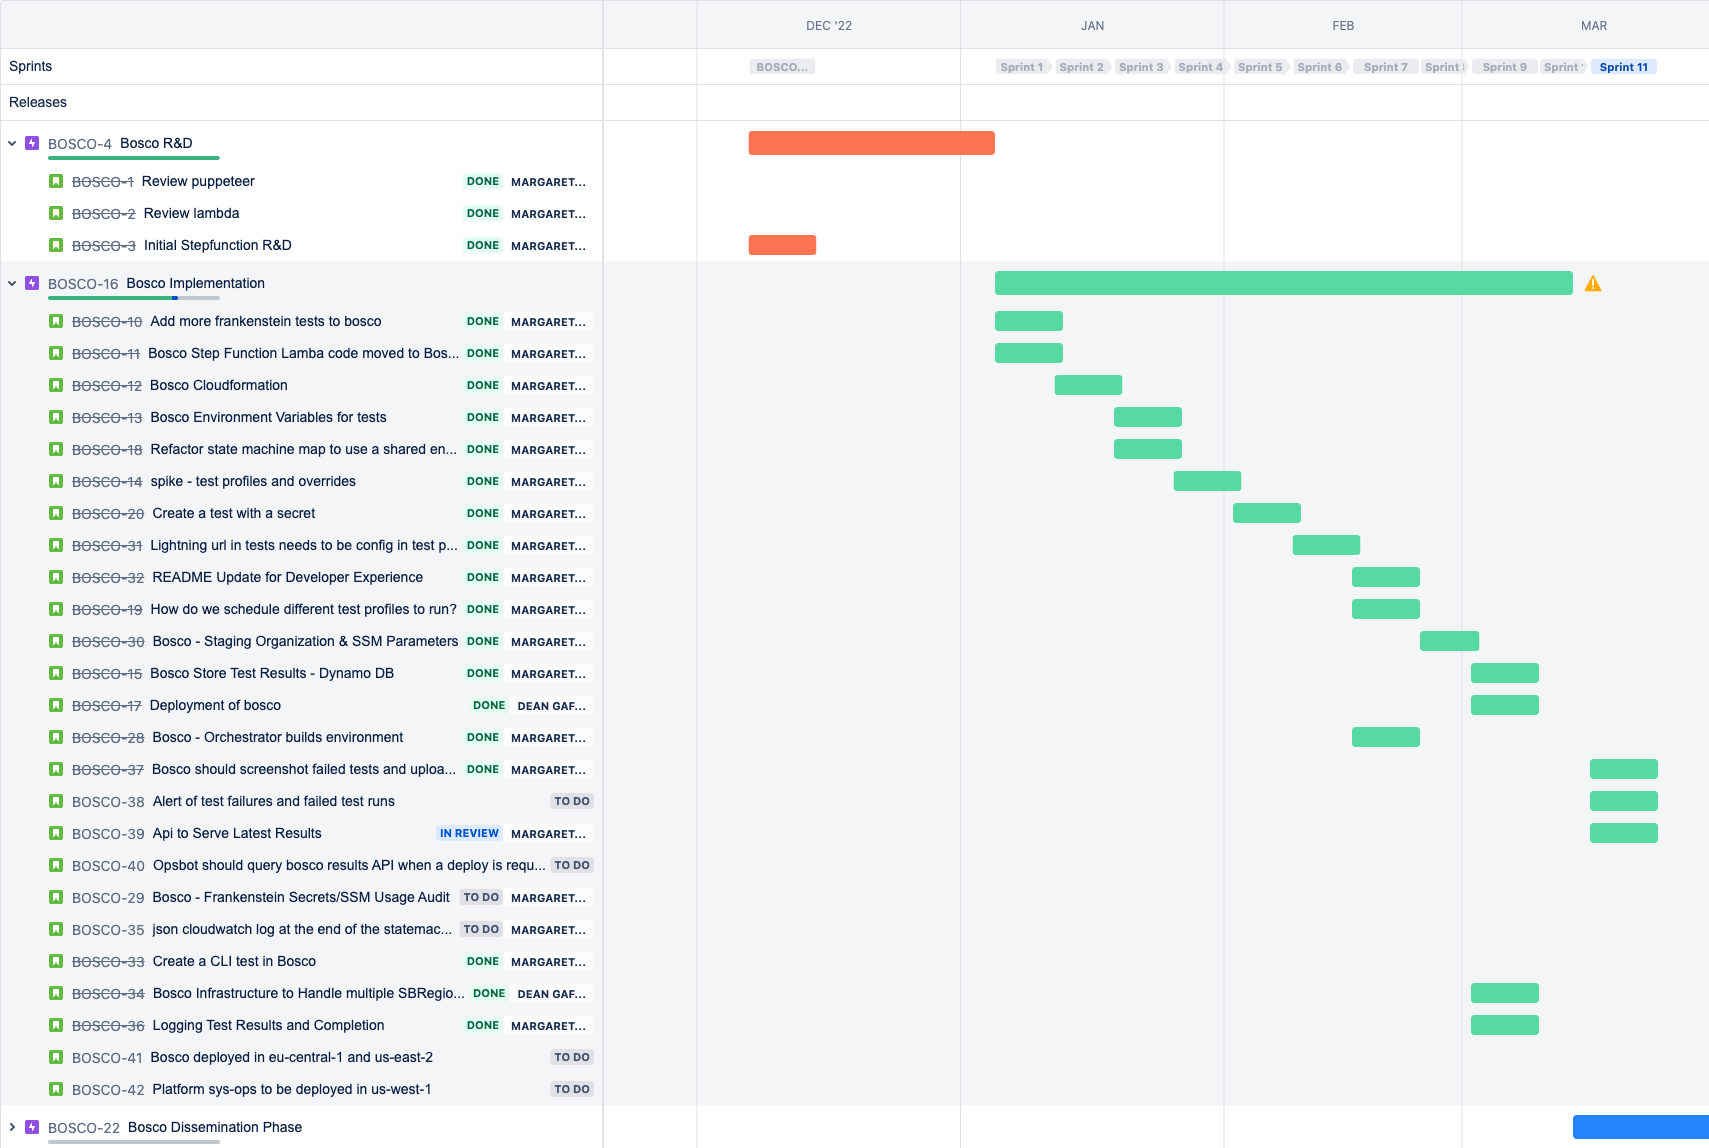
\includegraphics[width=15cm]{./diagrams/bosco_board.png}
 \caption{Bosco Jira Board: Sprint Planning}
\end{figure}

\chapter{Dependencies and Dev-Dependencies}
\subsection*{dependencies}
\begin{itemize}
  \item \textbf{@aws-sdk/client-dynamodb}: Amazon software package for DynamoDB.
  \item \textbf{@aws-sdk/lib-dynamodb}: Used in Bosco for Put command for writing to DynamoDB.
  \item \textbf{@servisbot/servisbot-cli}: The ServisBOT command line interface.
  \item \textbf{bluebird}: A fully featured promise library used in a test for delaying the test for 2 seconds.
  \item \textbf{cors}: A NodeJS package for providing Connect/Express middleware.
  \item \textbf{csv-parse}: For parsing JSON to CSV.
  \item \textbf{express}: A NodeJS framework for web development.
  \item \textbf{loglevel}: Logs context to the console and Cloudwatch.
  \item \textbf{luxon}: Immutable date wrapper.
  \item \textbf{number-to-words-en}: Transforms a number to words in English.
  \item \textbf{puppeteer}: Bosco's automation tool.
  \item \textbf{serverless-http}: For use with the API in a serverless environment.
  \item \textbf{sinon}: Test spies, stubs and mocks.
  \item \textbf{supertest}: Superagent driven library for testing HTTP servers.
\end{itemize}

\subsection*{dev-dependencies}
\begin{itemize}
  \item \textbf{aws-sdk}: Amazon software dependency kit.
  \item \textbf{depcheck}: a dependency check package which checks for unused dependencies before commits.
  \item \textbf{eslint}: a linting tool that ensures all the code is formatted consistently by anyone who makes changes to the code.
  \item \textbf{lambda-local}, a node module was used for testing purposes. This allowed for the running of the lamdas locally rather than having 
to deploy each time they were to be tested. 
  \item \textbf{mocha}: testing framework
  \item \textbf{pre-commit}: module to check for linting errors and dependency errors before committing to git.
\end{itemize}

\begin{figure}[H]
  \centering
  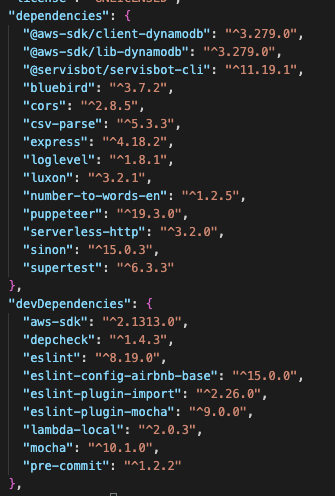
\includegraphics[width=11cm]{./diagrams/dependencies.png}
  \caption{dependencies and dev dependencies used for Bosco}
 \end{figure}

 \begin{table}[H]
  \centering
  \begin{tabular}{|c|c|c|c|}
  \hline \textbf
  \textbf{Time} & \textbf{TotalDurationInMs} & \textbf{SbRegion} & \textbf{Type} \\
  \hline 
  Mar 1, 2023 @ 12:06:29.052 & 319,344 & us1 & completion \\
  Mar 1, 2023 @ 12:07:40.376 & 401,819 & eu-1 & completion \\
  Mar 1, 2023 @ 12:10:42.724 & 598,784 & eu-private-1 & completion \\
  Mar 1, 2023 @ 12:14:59.371 & 218,456 & eu-1 & completion \\
  Mar 1, 2023 @ 12:16:07.944 & 320,090 & usscif1 & completion \\
  Mar 1, 2023 @ 12:16:09.875 & 301,098 & us1 & completion \\
  Mar 1, 2023 @ 12:17:27.389 & 398,329 & eu-private-1 & completion \\
  Mar 1, 2023 @ 12:26:32.122 & 322,127 & us1 & completion \\
  Mar 1, 2023 @ 12:27:25.214 & 390,314 & eu-1 & completion \\
  Mar 1, 2023 @ 12:30:51.696 & 602,877 & eu-private-1 & completion \\
  Mar 1, 2023 @ 12:34:58.503 & 218,544 & eu-1 & completion \\
  Mar 1, 2023 @ 12:35:32.092 & 282,295 & eu-private-1 & completion \\
  Mar 1, 2023 @ 12:36:28.552 & 343,885 & usscif1 & completion \\
  Mar 1, 2023 @ 12:36:28.624 & 319,462 & us1 & completion \\
  Mar 1, 2023 @ 12:46:36.648 & 326,957 & us1 & completion \\
  Mar 1, 2023 @ 12:47:23.415 & 386,681 & eu-1 & completion \\
  Mar 1, 2023 @ 12:50:51.373 & 608,557 & eu-private-1 & completion \\
  Mar 1, 2023 @ 12:55:00.374 & 220,826 & eu-1 & completion \\
  Mar 1, 2023 @ 12:55:58.806 & 311,210 & eu-private-1 & completion \\
  Mar 1, 2023 @ 12:56:36.230 & 325,104 & us1 & completion \\
  Mar 1, 2023 @ 12:56:38.795 & 354,038 & usscif1 & completion \\
  \hline
  \textbf{Average Time in ms} & 360,514 & & \\
  \hline
  \end{tabular}
  \caption{Frankenstein Test Runner times in ms over 1 hour}
  \label{tab:frank}
  \end{table}

\printbibliography[title={References}]

\chapter{Bibliography}
\textbf{Online}
\begin{enumerate}
\item https://www.opsramp.com/guides/aws-monitoring-tool/cloudwatch-synthetics/
\item https://www.functionize.com/automated-testing/assertion
\item https://jestjs.io
\item https://www.browserstack.com/guide/unit-testing-for-nodejs-using-mocha-and-chai
\item https://www.tricentis.com/blog/bdd-behaviour-driven-development
\item https://www.pluralsight.com/blog/software-development/tdd-vs-bdd
\item https://www.testim.io/blog/puppeteer-selenium-playwright-cypress-how-to-choose/
\item https://www.testim.io/blog/webinar-summary-is-ai-taking-over-front-end-testing/
\item https://aws.amazon.com/blogs/architecture/field-notes-scaling-browser-automation-with-puppeteer-on-aws-lambda-with-container-image-support/
\item https://moiva.io/
\item https://www.chaijs.com/api/assert/
\item https://docs.aws.amazon.com/AmazonCloudWatch/
\item https://docs.aws.amazon.com/lambda/latest/dg/gettingstarted-limits.html
\item https://oxylabs.io/blog/puppeteer-on-aws-lambda
\item https://aws.amazon.com/blogs/aws/new-for-aws-lambda-container-image-support/
\item https://www.npmjs.com/package/chrome-aws-lambda
\item https://www.docker.com/resources/what-container/
\item https://docs.aws.amazon.com/step-functions/latest/dg/concepts-input-output-filtering.html
\item https://blog.logrocket.com/testing-node-js-mocha-chai/
\item https://www.ponicode.com/shift-left/
\item https://www.tutorialspoint.com/puppeteer/
\item https://blog.shikisoft.com/3-ways-to-schedule-aws-lambda-and-step-functions-state-machines/
\item https://evanhalley.dev/post/aws-ssm-node/
\item https://dockerlabs.collabnix.com/beginners/components/what-is-container.html
\item https://www.youtube.com/watch?v=rQijrDj1wCQ
\item https://www.npmjs.com/
\item https://nodejs.org/
\item https://aws.amazon.com/blogs/containers/cross-region-replication-in-amazon-ecr-has-landed/
\end{enumerate}
\textbf{Paperback}
\begin{itemize}
  \item Rediscovering Javascript, Master ES6, ES7 and ES8. Author: Venkat Subramaniam. Edited by Jacquelyn Carter
\end{itemize}
\end{document}